% Preamble
\documentclass[11pt,dutch,parskip=half-]{scrartcl}

\usepackage{lmodern}
\usepackage{minted}
\usepackage{ugentassests2016}
\usepackage{graphicx}
\usepackage{array}
\usepackage{textcomp}
\usepackage{hyperref}
\usepackage{sidenotes}
\usepackage{enumitem}
\usepackage[Q=yes]{examplep}

\title{UGent-huisstijl}
\subtitle{Handleiding voor de \LaTeX-pakketten}
\author{Niko Strijbol}

\setcounter{tocdepth}{2}

% Document
\begin{document}
    \maketitle

    \begin{abstract}
        Deze verzameling pakketten en klassen voor \LaTeX\ geeft de mogelijkheid om verslagen, rapporten, werkstuken en boeken
        te maken met \LaTeX\ die voldoen aan de officiële huisstijl van de UGent.
    \end{abstract}

    \tableofcontents

    \section{Introductie}\label{sec:introductie}

    Deze handleiding volgt een \emph{top-down}-aanpak;
    we beginnen met de klassen die het vaakst gebruikt zullen worden, en gaan dan verder met de onderliggende pakketten.

    Deze handleiding is in het Nederlands.
    Een Engelse variant is in opbouw.

    \section{Installatie}\label{sec:installatie}
    De pakketten en klassen worden op de gewone wijze geïnstalleerd.
    De pakketten en klassen werken enkel met systemen die het pakket \texttt{fontspec} ondersteunen, zoals \texttt{lualatex}.

    Om ten volle te genieten van de huisstijl is het noodzakelijk het lettertype \emph{Panno Tekst UGent} te installeren of geïnstalleerd te hebben als systeemlettertype\footnote{Te downloaden op het intranet op \url{https://www.ugent.be/intranet/nl/op-het-werk/huisstijl/panno-lettertype.htm} }.

    \section{Taal}\label{sec:taal}
    De pakketten en klassen gebruiken de taal van het document voor het laden van de afbeeldingen.
    Vergelijk volgende resultaten:

    \vspace{\baselineskip}

    \begin{tabular}{ m{0.5\linewidth} m{0.5\linewidth} }
        \begin{minipage}[t]{0.5\linewidth}
            \begin{minted}{latex}
\documentclass[11pt, dutch]{article}
\usepackage{graphicx, ugentassests2016}
\begin{document}
    \includegraphics{\ugentdefault}
\end{document}
            \end{minted}
        \end{minipage}
        & \begin{minipage}{.5\linewidth}
            \includegraphics[width=\linewidth]{\ugentdefaultnl}
        \end{minipage} \\
    \end{tabular}

    \begin{tabular}{ m{0.5\linewidth} m{0.5\linewidth} }
        \begin{minipage}[t]{0.5\linewidth}
            \begin{minted}{latex}
\documentclass[11pt, english]{article}
\usepackage{graphicx, ugentassests2016}
\begin{document}
    \includegraphics{\ugentdefault}
\end{document}
            \end{minted}
        \end{minipage}
        & \begin{minipage}{.5\linewidth}
              \includegraphics[width=\linewidth]{\ugentdefaulten}
        \end{minipage} \\
    \end{tabular}

    \section{Klassen \texttt{ugentreport2016}, \texttt{ugentbook2016} en \texttt{ugentarticle2016}}\label{sec:klassen}

    Deze pakketten zijn bedoeld als aanvulling op de \KOMAScript-klassen.
    Bijgevolg zijn er drie documentklassen, die aansluiten bij die voorzien door \KOMAScript:

    \begin{itemize}
        \item \texttt{ugentreport2016} gebruikt \texttt{scrreprt} als onderliggende klasse.
        \item \texttt{ugentbook2016} gebruikt \texttt{scrbook} als onderliggende klasse.
        \item \texttt{ugentarticle2016} gebruikt \texttt{scrartcl} als onderliggende klasse.
    \end{itemize}

    Alle klassen ondersteunen dezelfde opties, de enige verschillen zijn de onderliggende klassen en de standaardwaarden van de opties.

    Snel op weg is mogelijk door het \texttt{example.tex}-bestand te gebruiken, dat de meeste opties kort uitlegt.

    \subsection{Gebruik}\label{subsec:gebruik}
    
    De klassen worden gebruikt zoals elke andere documentklasse:
    \begin{minted}{latex}
\documentclass[11pt,campus=default,faculty=we,layout=all]{ugentreport2016}
    \end{minted}

    Er zijn enkele opties specifiek voor onze klassen, beschreven in sectie~\ref{subsec:opties}.
    Alle andere opties worden doorgegeven aan de onderliggende klasse.
    Wie zijn document grondig wilt aanpassen kijkt daarom best ook naar de \KOMAScript-handleiding.

    \subsection{Opties}\label{subsec:opties}

    De klassen hebben vijf opties, in \emph{key-value}-formaat.

    \subsubsection{\texttt{campus=\textlangle default|kortrijk|global\textrangle}}\label{subsubsec:campus}

    Stelt in welk logo gebruikt moet worden.
    De drie opties zijn beschreven in tabel~\ref{table:campus}.

    \begin{table}
        \begin{center}
            \caption{Overzicht waarden \texttt{campus}\label{table:campus}}
            \begin{tabular}{l l}
                \hline
                Waarde & Voorbeeld \\
                \hline
                \texttt{default}  &
                \begin{minipage}{.3\textwidth}
                    \includegraphics[width=\linewidth]{\ugentdefault}
                \end{minipage} \\
                \texttt{kortrijk} &
                \begin{minipage}{.3\textwidth}
                    \includegraphics[width=\linewidth]{\ugentkortrijk}
                \end{minipage} \\
                \texttt{global} &
                \begin{minipage}{.3\textwidth}
                    \includegraphics[width=\linewidth]{\ugentglobal}
                \end{minipage} \\
                \hline
            \end{tabular}
        \end{center}
    \end{table}

    Merk op dat de campussen Kortrijk en Global geen vertaalde logo's hebben.

    \subsubsection{\texttt{faculty=\textlangle faculteitscode\textrangle}}\label{subsubsec:faculty}
    Deze optie neemt een tweeletterige code van de faculteit.
    Een lijst van deze afkortingen is te vinden in tabel~\ref{table:faculty}.
    De optie beïnvloed het facultaire logo alsook de facultaire kleuren die eventueel gebruikt worden.

    \begin{table}
        \begin{center}
            \caption{Afkortingen van de faculteiten\label{table:faculty}}
            \begin{tabular}{l l}
                \hline
                Afkorting & Volledige naam \\
                \hline
                \texttt{we} & Faculteit Wetenschappen \\
                \texttt{re} & Faculteit Recht en Criminologie \\
                \texttt{lw} & Faculteit Letteren en Wijsbegeerte \\
                \texttt{ge} & Faculteit Geneeskunde en Gezondheidswetenschappen \\
                \texttt{ea} & Faculteit Ingenieurswetenschappen en Architectuur \\
                \texttt{eb} & Faculteit Economie en Bedrijfskunde \\
                \texttt{di} & Faculteit Dierengeneeskunde \\
                \texttt{pp} & Faculteit Psychologie en Pedagogische Wetenschappen \\
                \texttt{bw} & Faculteit Bio-Ingenieurswetenschappen \\
                \texttt{fw} & Faculteit Farmaceutische Wetenschappen \\
                \texttt{ps} & Faculteit Politieke en Sociale Wetenschappen \\
                \texttt{none} & Speciale waarden, geen faculteit \\
                \hline
            \end{tabular}
        \end{center}
    \end{table}

    \subsubsection{\texttt{footer=\textlangle true|false\textrangle}}
    De optie \texttt{footer} geeft aan of de voettekst moet toegevoegd worden of niet.
    Standaard staat deze optie uit, tenzij de optie \texttt{ugentstyle} de waard \texttt{notes} krijgt.
    In dat geval wordt de voettekst wel getoond.

    \subsubsection{\texttt{ugentstyle=\textlangle course|report|notes\textrangle}}\label{subsubsec:style}

    Deze optie is vooral van invloed op het type voorblad dat gegenereerd wordt.
    Gebruik \texttt{course} voor een voorblad zoals in een boek, \texttt{report} is geschikt voor rapporten, thesissen, werkstukken, enz.
    \texttt{notes} is ten slotte aangewezen voor verslagen, notulen, administratieve documenten, enz.
    Deze laatste optie gebruikt naast een ander voorblad ook een andere voettekst.
    Een voorbeeld van deze stijlen is te vinden in bijlagen~\ref{sec:voorblad-met-stijl-course},~\ref{sec:voorblad-met-stijl-report}~en~\ref{sec:voorblad-met-stijl-notes}.

    \subsubsection{\texttt{layout=\textlangle stijlniveau\textrangle}}

    Deze optie duidt aan tot welk niveau het document opgemaakt moet worden naar de normen van de huisstijl.
    Elk volgend niveau past ook de opmaak van het vorige niveau toe.
    Zo zal niveau 3 ook de opmaak van niveau 2 en niveau 1 toepassen.
    De hiërarchie ziet er als volgt uit: \texttt{none} → \texttt{margins} → \texttt{colours} → \texttt{titlestyle} → \texttt{titlefont} → \texttt{all}.

    \begin{enumerate}
        \item \textbf{\texttt{none}} -- Pas geen opmaak toe buiten de titelpagina. Dit is de standaardwaarde.
        \item \textbf{\texttt{margins}} -- Pas de marges van het document aan.
        \item \textbf{\texttt{colours}} -- Pas kleuren toe. Concreet betekent dit dat de titels van het document in het blauw zullen zijn.
        \item \textbf{\texttt{titlestyle}} -- Maak de titels op. Hierbij gaat het om het omzetten naar hoofdletters en onderlijnen van de titels.
        \item \textbf{\texttt{titlefont}} -- Pas het lettertype toe op de titels.
        \item \textbf{\texttt{all}} -- Pas alles toe. Concreet zal dit ervoor zorgen dat alle lettertypes voldoen aan de huisstijl. Omdat de UGent geen licentie heeft om het hoofdlettertype (Panno Tekst) te gebruiken voor schuine letters of cursief, wordt het secundaire lettertype gebruikt voor de hoofdtekst, namelijk \textit{Arial}.
    \end{enumerate}

    \section{Pakket \texttt{ugentstyle2016}}\label{sec:pakkettexttt}
    Dit is het pakket dat verantwoordelijk is voor het voorblad.

    \subsection{Opties}\label{subsec:opties2}
    Het pakket heeft volgende opties, de reeds hierboven beschreven zijn:
    \begin{itemize}
        \item \textbf{\texttt{style}} -- Zie deel~\ref{subsubsec:style}. De standaardwaarde is \texttt{course}.
        \item \textbf{\texttt{faculty}} -- Zie deel~\ref{subsubsec:faculty}. Standaardfaculteit is \texttt{we}.
        \item \textbf{\texttt{campus}} -- Zie deel~\ref{subsubsec:campus}. Standaardwaarde is \texttt{default}.
    \end{itemize}

    \subsection{Metagegevens}\label{subsec:metagegevens}
    Om het voorblad van data te voorzien zijn er een heleboel commando's analoog aan \mintinline{latex}{\author{}} en verwanten.
    Afhankelijk van het type voorblad worden gegevens op een andere plaats getoond of zelfs niet getoond.
    Een visueel overzicht wordt gegeven in bijlagen~\ref{sec:voorblad-met-stijl-course},~\ref{sec:voorblad-met-stijl-report}~en~\ref{sec:voorblad-met-stijl-notes}.
    Tabel~\ref{table:titlemeta} bevat een beschrijving van alle beschikbare commando's.

    \begin{table}
        \begin{center}
            \caption{Beschikbare commando's voor het titelblad\label{table:titlemeta}}
            \begin{tabular}{p{0.2\linewidth} p{0.7\linewidth}}
                \hline
                Commando & Betekenis en gebruik \\
                \hline
                \verb|\author{}| & Zoals in standaard\LaTeX \\
                \verb|\title{}|  & Zoals standaard\LaTeX \\
                \verb|\subtitle{}| & Zoals standaard-\KOMAScript \\
                \verb|\academyyear{}| & Het academiejaar, bv. 2017 -- 2018. \\
                \verb|\programme{}| & De richting, bv. Informatica. \\
                \verb|\wordcount{}| & Aantal woorden in het werk.\footnote{Dit wordt misschien ooit automatisch berekened.} \\
                \verb|\studentnumber{}| & Studentennummer. \\
                \verb|\email{}| & E-mailadres van de auteur. \\
                \verb|\phone{}| & Telefoonnummer van de auteur. \\
                \verb|\address{}| & Adres van de auteur. Kan over meerdere regels. \\
                \verb|\department{}| & Departement/vakgroep binnen de faculteit. \\
                \verb|\researchgroup{}| & Onderzoeksgroep. \\
                \verb|\facultisch{}| & De faculteit (of aanverwanten, zoals Directie ICT). Standaard wordt dit de naam van de faculteit. Als \texttt{faculty=none}, moet dit gegeven worden. \\
                \verb|\titletext{}| & Vrije, niet opgemaakte tekst voor op het titelblad. \\
                \hline
            \end{tabular}
        \end{center}
    \end{table}

    Ze worden gebruikt zoals de normale \LaTeX-commando's:
    \begin{minted}{latex}
\author{Jan Jaap}
\title{Een mooie paper}
\subtitle{Zonder toegevoegde data}
    \end{minted}

    \section{Pakket \texttt{ugentassets2016}}\label{sec:pakkettexttt2}
    Dit pakket voorziet de logo's, kleuren en andere \emph{assets}.
    Als voorbeeld wordt in dit deel vaak de Faculteit Wetenschappen gebruikt.

    \subsection{Logo's}\label{subsec:logos}

    Het pakket heeft commando's die het pad naar de verschillende logo's geven.
    Deze kunnen dan gebruikt worden om bijvoorbeeld de logo's te tonen:

    \begin{minted}{latex}
\includegraphics{\ugentdefault}
    \end{minted}

    Zoals vermeld in deel~\ref{sec:taal} worden de logo's automatisch aangepast aan de taal.
    Er zijn wel experimentele\footnote{Dit betekent dat ze kunnen veranderen of verdwijnen.} versies van de commando's die altijd hetzelfde logo teruggeven.
    Om ze te gebruiken voegt men de tweeletterige taalcode toe aan het commando:

    \begin{minted}{latex}
\ugentdefault       % afhankelijk van taal
\ugentdefaultnl     % altijd Nederlands
\ugentdefaulten     % altijd Engels
    \end{minted}

    Volgende commando's zijn beschikbaar:

    \begin{description}[style=nextline]
        \item[\Q{\\ugentdefault}] Geeft het gewone logo van de Universiteit.
                Rond dit, en andere logo's, is witruimte voorzien.
            \begin{marginfigure}[-1cm]\includegraphics[width=\marginparwidth]{\ugentdefault}\end{marginfigure}
        \item[\Q{\\ugentkortrijk}] Logo van de Campus Kortrijk.
                Dit logo heeft geen vertaling.
            \begin{marginfigure}[-0.5cm]\includegraphics[width=\marginparwidth]{\ugentkortrijk}\end{marginfigure}
        \item[\Q{\\ugentglobal}] Logo van de Global Campus.
                Dit logo heeft geen vertaling.
            \begin{marginfigure}[-0.5cm]\includegraphics[width=\marginparwidth]{\ugentglobal}\end{marginfigure}
        \item[\Q{\\ugentfacultylogo{code}}] Geeft het logo van de faculteit.
                De parameter \texttt{code} is de tweeletterige code uit tabel~\ref{table:faculty}.
                Merk op dat de speciale waarde \texttt{none} niet werkt in deze marco.
            \begin{marginfigure}[-0.5cm]\includegraphics[width=\marginparwidth]{\ugentfacultylogo{we}}\end{marginfigure}
    \end{description}

    \subsection{Kleuren}\label{subsec:kleuren}

    Ook alle officiële kleuren van de UGent zijn beschikbaar. Deze kleuren zijn gedefinieerd als een \LaTeX-kleur, en
    kunnen dus overal gebruikt worden:

    \begin{tabular}{ m{0.5\linewidth} m{0.5\linewidth} }
        \begin{minipage}[t]{0.5\linewidth}
            \begin{minted}{latex}
{\color{ugent-blue} Dit is blauw.}
            \end{minted}
        \end{minipage}
        & \begin{minipage}{.5\linewidth}
              {\color{ugent-blue} Dit is blauw.}
        \end{minipage} \\
    \end{tabular}

    Een lijst van beschikbare kleuren:

    \begin{description}[style=nextline]
        \item[\Q{ugent-blue}] Officiële blauwe hoofdkleur. \begin{marginfigure}{\textcolor{ugent-blue}{\rule{0.5cm}{0.5cm}}}\end{marginfigure}
        \item[\Q{ugent-yellow}] Officiële gele accentkleur. \begin{marginfigure}{\textcolor{ugent-yellow}{\rule{0.5cm}{0.5cm}}}\end{marginfigure}
        \item[\Q{ugent-{code}}] Officiële faculteitskleur.
                De parameter \texttt{code} is de tweeletterige code uit tabel~\ref{table:faculty}.
                Merk op dat de speciale waarde \texttt{none} niet werkt in deze marco.
            \begin{marginfigure}{\textcolor{ugent-we}{\rule{0.5cm}{0.5cm}}}\end{marginfigure}
    \end{description}

    \subsection{Lettertypes}\label{subsec:lettertypes}

    Het pakket laadt het lettertype \emph{Panno Tekst UGent} in met \texttt{fontspec}.
    Dit is beschikbaar met \mintinline{latex}{\pannofamily}.
    Zoals reeds vermeld vereist dit uiteraard dat Panno geïnstalleerd is als systeemlettertype\footnote{Technisch moet het lettertype \emph{known} zijn voor \texttt{fontspec}}.
    Verder zijn er twee commando's die het leven gemakkelijker maken om het lettertype te gebruiken.

    \begin{description}[style=nextline]
        \item[\Q{\\panno[grootte1][grootte2]{tekst}}] Zet de \texttt{tekst} in Panno, met groottes \texttt{grootte1} en \texttt{grootte2}. Deze grotes worden gebruikt bij het \mintinline{latex}{\fontsize{groott1}{grootte2}}-commando.
        \item[\Q{\\pannosemibold[grootte1][grootte2]{tekst}}] Zet de \texttt{tekst} in Panno Semi Bold, met groottes \texttt{grootte1} en \texttt{grootte2}. Deze grotes worden gebruikt bij het \mintinline{latex}{\fontsize{groott1}{grootte2}}-commando.
    \end{description}

    Het gebruik is eenvoudig:

    \begin{tabular}{ m{0.6\linewidth} m{0.4\linewidth} }
        \begin{minipage}[t]{0.6\linewidth}
            \begin{minted}{latex}
% Puur fontspec-commando
{\pannofamily Dit is Panno.}
% Hulpcommando's
\panno[16pt][30pt]{Panno Tekst}
\pannosemibold[16pt][30pt]{Panno Tekst}
            \end{minted}
        \end{minipage}
        & \begin{minipage}[t]{\linewidth}
            \vspace{0.45\baselineskip}
            {\pannofamily Dit is Panno.} \par
            \vspace{\baselineskip}
              \panno[16pt][30pt]{Panno Tekst} \par
              \pannosemibold[16pt][30pt]{Panno Tekst}
        \end{minipage} \\
    \end{tabular}

    \vspace{\baselineskip}
    Tot slot opnieuw opmerken dat cursieve varianten van dit lettertype niet bestaan.

    \subsection{Namen der faculteiten}\label{subsec:namen-der-faculteiten}

    Er is een commando dat de vertaalde naam van de faculteit geeft: \mintinline{latex}{\ugentfacultyname{code}}.
    Hierbij is \texttt{code} opnieuw de tweeletterige code uit tabel~\ref{table:faculty}.
    Deze macro werkt ook niet als \texttt{faculty=none}.
    Hiervoor is (nog) geen vast commando voorzien; de naam zal altijd afhangen van de taal van het document.

    \begin{tabular}{ m{0.6\linewidth} m{0.4\linewidth} }
        \begin{minipage}[t]{0.6\linewidth}
            \begin{minted}{latex}
\ugentfacultyname{we} \par
\ugentfacultyname{re}
            \end{minted}
        \end{minipage}
        & \begin{minipage}[t]{\linewidth}
              \ugentfacultyname{we} \par
              \ugentfacultyname{re}
        \end{minipage} \\
    \end{tabular}

    \subsection{Grid}\label{subsec:grid}

    De huisstijl definieert een typografisch grid over de pagina\footnote{Zie \url{https://styleguide.ugent.be/basisprincipes/grid-en-lay-out.html}}, dat bekomen wordt door de lengte door 7 te delen.
    Dat zijn de grote blokken.
    De lengte van een groot blok wordt dan gedeeld door 4 om een klein blok te krijgen.
    Het kleine blok is de basisgrootte van het document.
    Pakketten zoals \texttt{ugentstyle2016} gebruiken deze basisgrootte om de positie van onderdelen te bepalen.
    Er zijn twee macro's beschikbaar, \mintinline{latex}{\bigblock} en \mintinline{latex}{\smallblock}, die de lengte van respectievelijk het grote en het kleine blok geven.
    Dit zijn lengtes en kunnen dus overal gebruikt worden waar lengtes toegelaten worden.

    \begin{minted}{latex}
% Lengte zal 3*(lengte blad/28) zijn
\includegraphics[width=3\smallblock]{\ugentkortrijk}
    \end{minted}

    \appendix

    \section{Voorblad met stijl \texttt{course}}\label{sec:voorblad-met-stijl-course}
    \begin{center}
        \frame{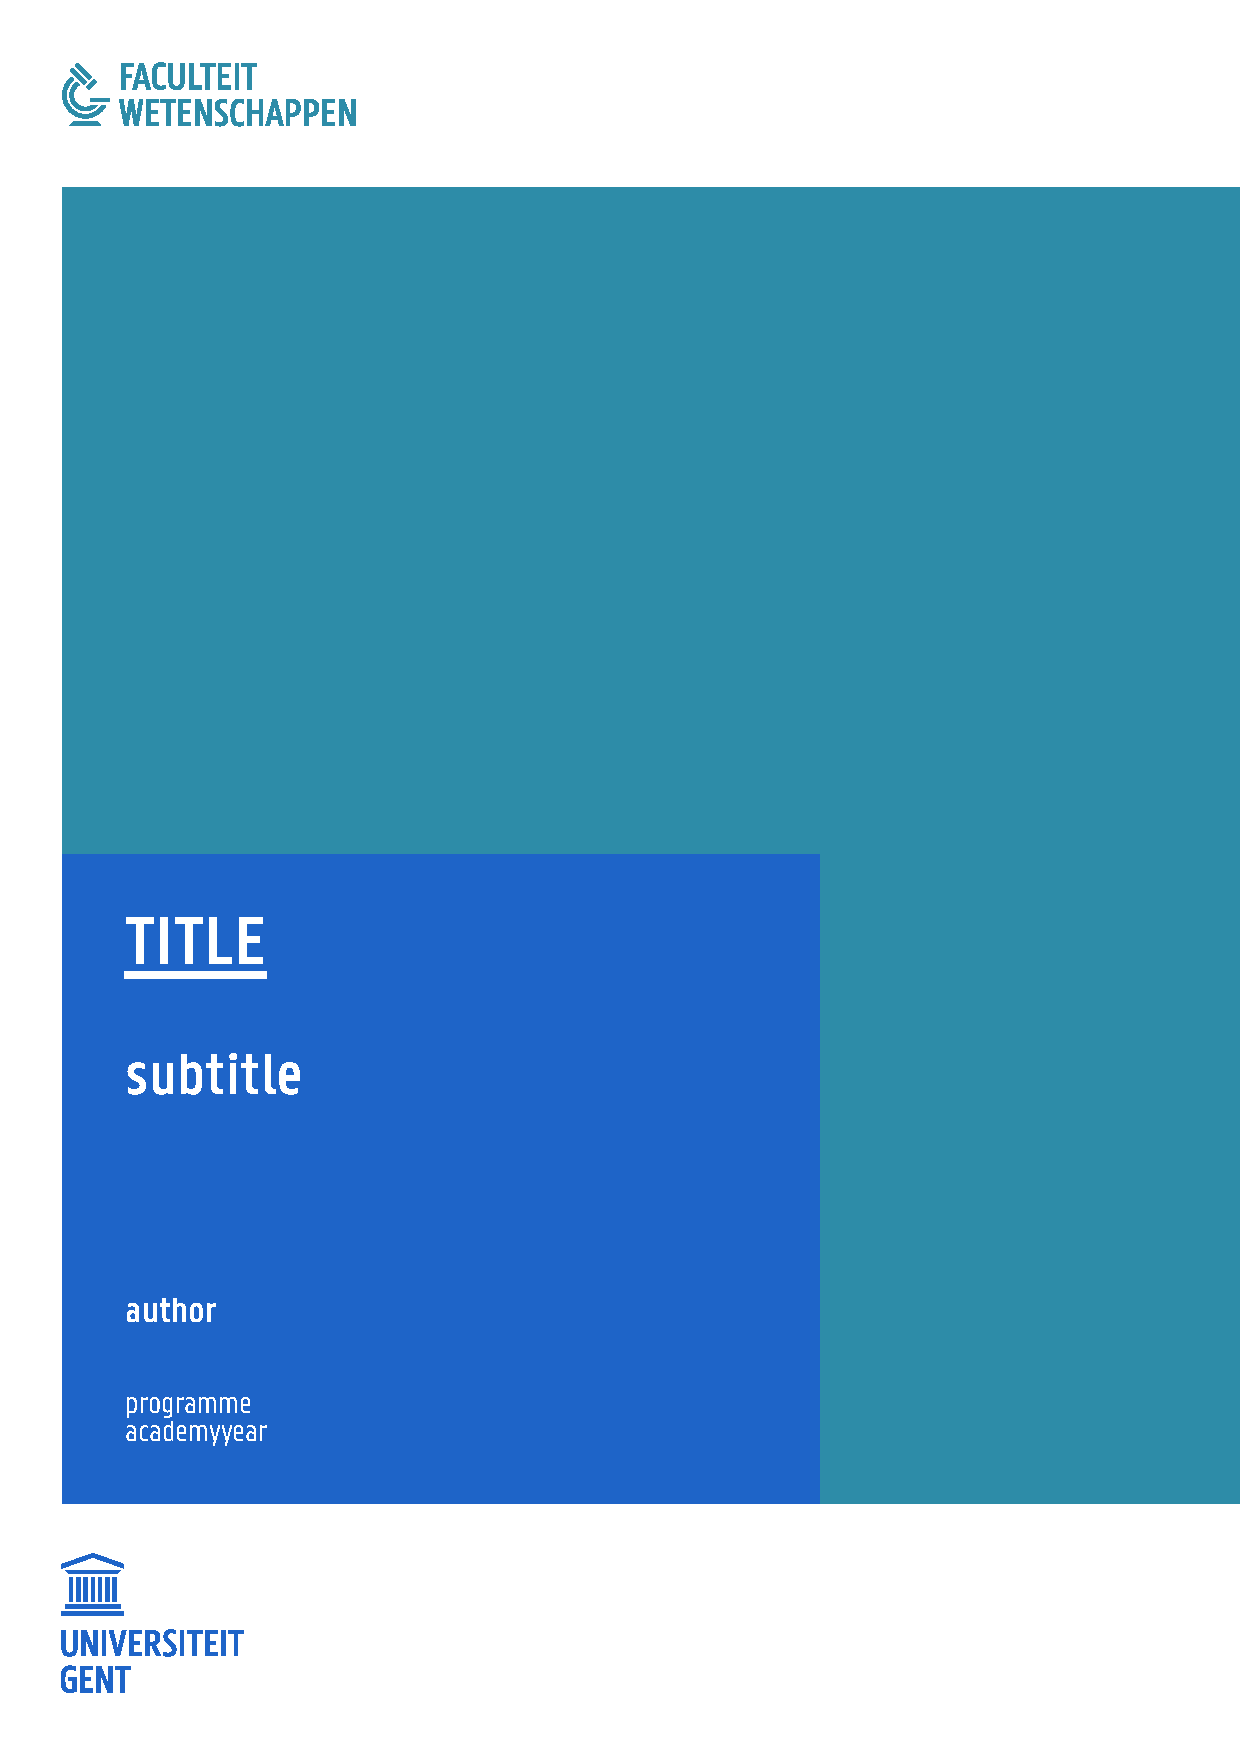
\includegraphics[width=0.9\textwidth]{frontpages/ugent2016title-course.pdf}}
    \end{center}

    \section{Voorblad met stijl \texttt{report}}\label{sec:voorblad-met-stijl-report}
    \begin{center}
        \frame{
\includegraphics[width=0.9\textwidth]{frontpages/ugent2016title-report.pdf}}
    \end{center}

    \section{Voorblad met stijl \texttt{notes}}\label{sec:voorblad-met-stijl-notes}
    \begin{center}
        \frame{
\includegraphics[width=0.9\textwidth]{frontpages/ugent2016title-notes.pdf}}
    \end{center}

    \section{Wijzigingen}

    Dit onderdeel bevat de voornaamste wijzigingen.
    De exacte wijzigingen kunnen gevonden worden in de Github-repository van de pakketten.

    \subsubsection*{15 februari 2019}
    \begin{itemize}
        \item Bugfixes bij onderlijnen lange titels
        \item Voeg klasse \texttt{ugentartcl2016} toe
    \end{itemize}

\end{document}
